\chapter{Distribución Weibull}

El presente capítulo tiene como objetivo principal proponer una reparametrización de la distribución Weibull para adaptarla al modelo de regresión cuantílica. Para dicha reparametrización, se definirá su función de densidad y función acumulada, y asimismo se examinará sus propiedades.

\section{Distribución Weibull}

La distribución Weibull fue presentada por \cite{weib:weib}. En dicho artículo de investigación, Weibull menciona las características de una función de densidad suficientemente flexible para ser adaptada a diversas investigaciones, desde la rama de resistencia de materiales hasta el análisis de altura de hombres adultos radicados en las Islas Británicas. Una variable aleatoria continua $Y$, con soporte $Y \in [0,\infty]$, sigue una distribución Weibull si su función de densidad es dada por la siguiente expresión:

\begin{equation*}
f{(y)}= \frac{\alpha}{\sigma}\left(\frac{y}{\sigma}\right)^{\alpha-1} \exp{\left(-\frac{y}{\sigma}\right)^{\alpha}}
\end{equation*}

\noindent en dónde $\alpha$ corresponde al parámetro de escala, con $\alpha > 0$, y $\sigma$ corresponde al parámetro de forma, con $\sigma > 0$. La notación de una variable aleatoria $Y$ que sigue esta distribución se indica como $Y \sim W(\alpha,\sigma)$. La función de densidad acumulada de $Y$ tiene la siguiente expresión:

\[F{(y)}=1-\exp^{-{(\frac{y}{\sigma})}^{\alpha}}.\]

\noindent Asimismo, su función de cuantiles es dada por:

\[q_{t}=\sigma{(-\log{(1-t)})}^{\frac{1}{\alpha}}\]

\noindent para $0 < t < 1$.

La flexibilidad denotada por Weibull puede observarse a través de la figura 1, en dónde se observa que el parámetro de forma permite ..... Asimismo, el parámetro de escala permite identificar lo junta que puede ser la distribución,

Para una variable $Y \sim W(\alpha, \sigma)$, la media y varianza se define de la siguiente forma:

\[E(Y)=\sigma \Gamma\left( 1+\frac{1}{\alpha} \right).\]
\[V(Y)=\sigma^{2}\left[ \Gamma\left( 1+\frac{2}{\alpha} \right)-\left( \Gamma\left( 1+\frac{1}{\alpha} \right) \right)^{2} \right].\]

\subsection{Proposición de una nueva estructura de la distribución}

Consideramos una reparametrización del parámetro de forma $\sigma$ en términos del cuantil $t, q_{t}$ en los siguientes términos:

\[q_{t}=\sigma\left( -\log\left( 1-t \right) \right)^{\frac{1}{\alpha}}.\]

\noindent en dónde $t$ será un valor conocido y se encuentra en el intervalo $[0,1]$. En esta nueva esctructura, $q_{t}$ y $\alpha$ tienen espacios paramétricos independientes tal que $(q_{t},\alpha) \in (0,\infty)$ x $(0,\infty)$. Una variable aleatoria que sigue esta parametrización se denota como $Y \sim W_{r}(q_{t},\alpha)$.

La función de densidad de dicha variable $Y$ tiene la siguiente expresión:
\begin{equation}
f_{Y}(y| q_{t},\alpha)=\frac{\alpha c(t)}{q_{t}}\left( \frac{y}{q_{t}} \right)^{\alpha-1}\exp\left( -c(t)\left( \frac{y}{q_{t}} \right)^{\alpha} \right)
\end{equation}
\\
\noindent en dónde $c(t)= \left( -\log(1-t) \right)^{\frac{1}{\alpha}}$. Los parámetros $q_{t}$ y $\alpha$ caracterizan la función de densidad conforme se observa el gráfico siguiente:

\textbf{Nota del profesor Valdivieso: Mejorar esta densidad.}

\begin{figure}[H]
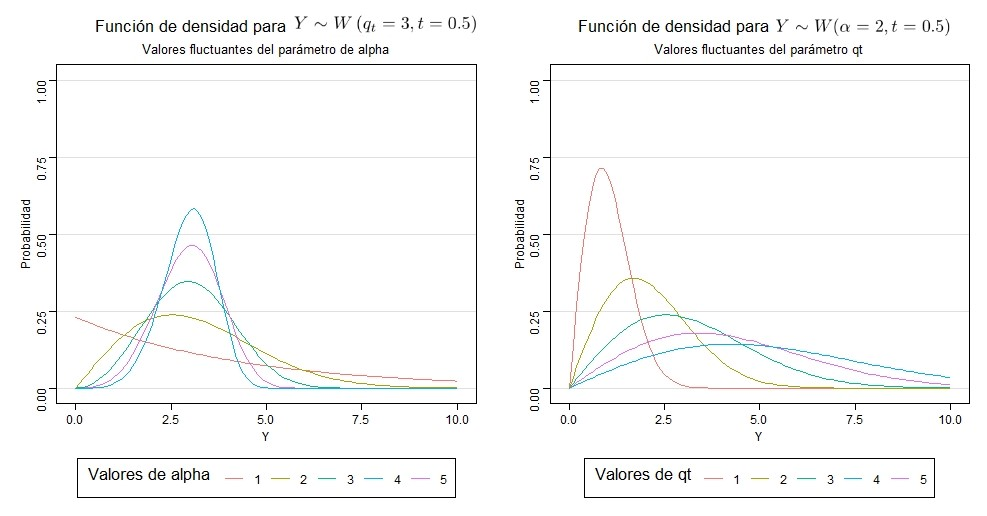
\includegraphics[width=\textwidth]{densidad1}
\caption{Función de densidad de una distribución Weibull bajo la reparametrización propuesta.}
\end{figure}

\noindent Se observa que en la medida que $q_{t}$ aumenta, la distribución incrementa su asimetría hacia la derecha. Ello también sucede, aunque en menor grado, cuando $\alpha$ aumenta. No obstante, se observa que en la medida que $\alpha$ tiende a 0, incrementa la dispersión.

Reexpresando la función acumulada en los términos de la parametrización propuesta, esta tendría la siguiente forma:
\begin{equation} \label{eq:1}
F_{Y}\left(y| q_{t},\alpha,t \right)=1-\exp\left( -c(t)\left( \frac{y}{q_{t}} \right)^{\alpha} \right).
\end{equation}
\subsection{Estudio de la parametrización propuesta}

La esperanza y varianza de una variable aleatoria bajo la parametrización Weibull propuesta están dadas bajo la siguiente expresión:
\begin{equation}
E(Y)=\frac{q_{t}}{c(t)^{\frac{1}{\alpha}}}\Gamma\left( 1+\frac{1}{\alpha} \right)
\end{equation}

\begin{equation}
Var(Y)=\frac{q_{t}^{2}}{c(t)^{\frac{1}{\alpha}}}\left[ \Gamma\left( 1+\frac{2}{\alpha}\right)-\Gamma\left( 1+\frac{1}{\alpha} \right)^{2} \right]
\end{equation}

Bajo la parametrización propuesta, se observa que para un $\alpha$ fijo el valor esperado se comporta de forma lineal en la medida que aumente el parámetro $q_{t}$ conforme se observa en el cuadro siguiente:

\textbf{Nota del profesor Valdivieso: Mejorar esta densidad.}

\begin{figure}[H]
	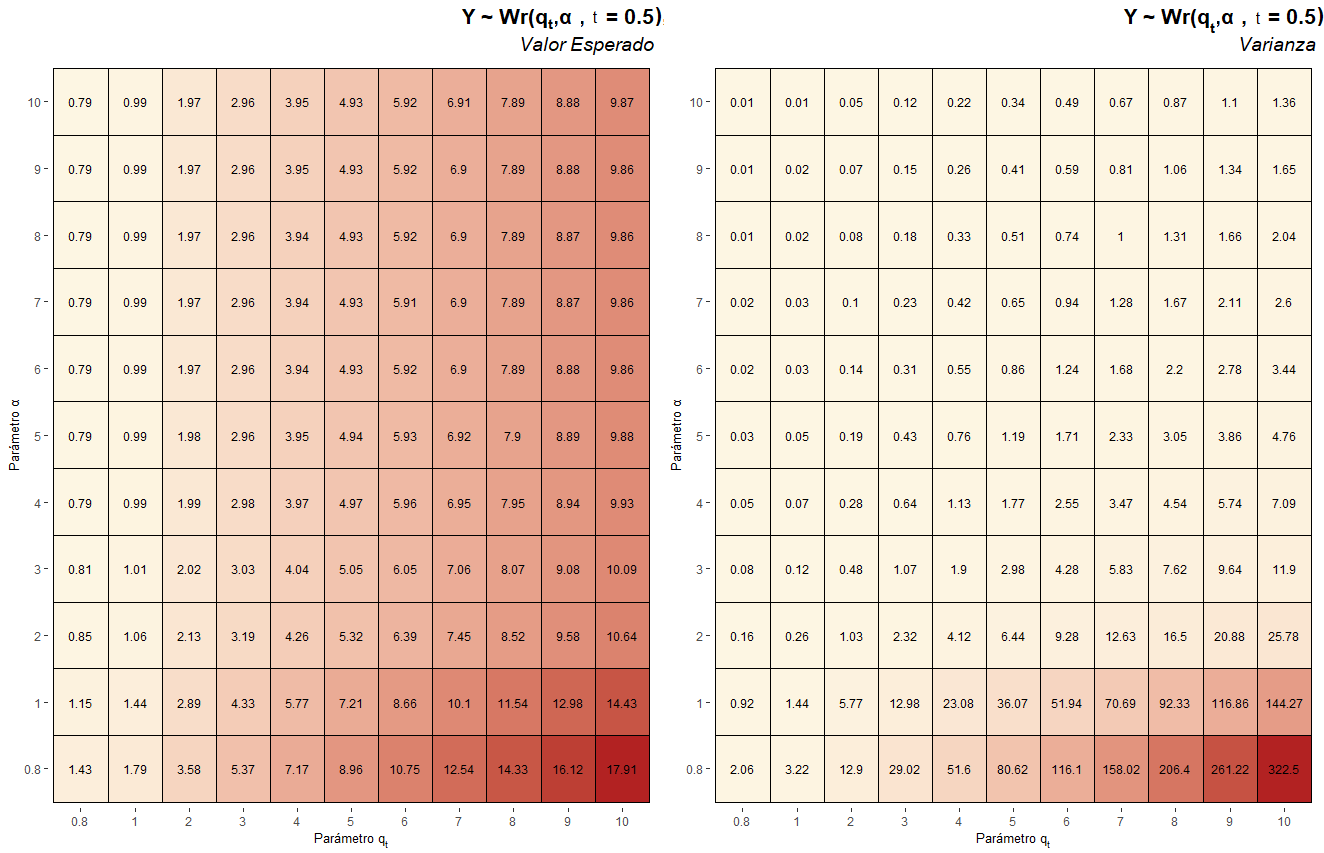
\includegraphics[width=\textwidth]{esperado}
	\caption{Valor esperado de una distribución Weibull bajo la parametrización propuesta.}
\end{figure}
\noindent No obstante, para un $q_{t}$ fijo, lo mismo no se observa en la medida que aumente $\alpha$. Se observa un comportamiento no lineal y asintótico: cuando $\alpha$ tiende a 0, el valor esperado tiende a infinito. Cuando $\alpha$ aumenta, el valor esperado se estabiliza.

En el caso de la varianza se observa que para un $\alpha$ fijo, en la medida que aumente el parámetro $q_{t}$ la varianza aumenta de forma exponencial. No obstante, y como se puede apreciar cuando $q_{t}$ está fijo, en la medida que los valores de $\alpha$ sean pequeños, la varianza incrementa drásticamente. Asimismo, como se aprecia en el cuadro adjunto, la varianza tiende a 0 en la medida que $\alpha$ aumente.

\begin{figure}[H]
	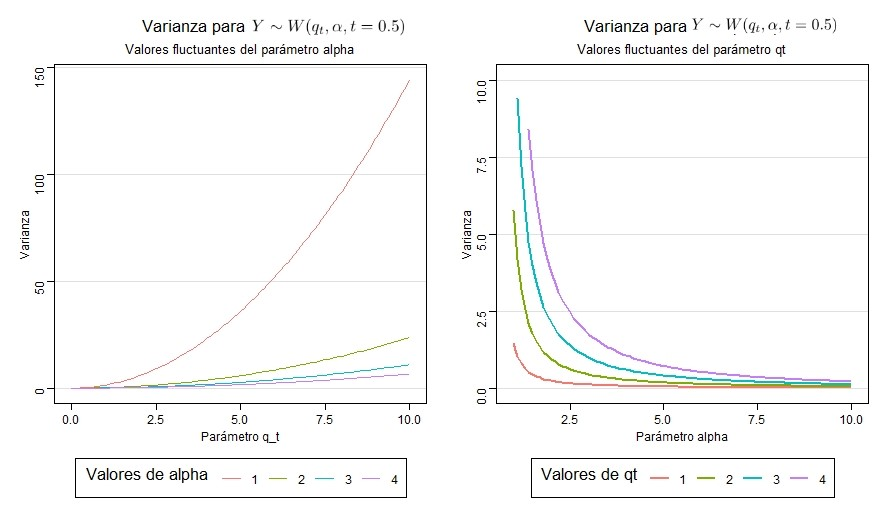
\includegraphics[width=\textwidth]{varianza}
	\caption{Varianza bajo la parametrización propuesta.}
\end{figure}
